\documentclass[12pt,a4paper,openany,oneside]{book}

\usepackage{framed}
\usepackage{xcolor}
\usepackage{hyperref}
\usepackage[utf8]{inputenc}
\usepackage[italian]{babel}
\usepackage{graphicx}
\usepackage{amsmath}
\usepackage{amsfonts}
\usepackage{float}
\usepackage{listings}
\usepackage{courier}
\lstset{
    language=C++,
    basicstyle=\footnotesize\ttfamily,
    numbers=left,
    numberstyle=\tiny,
    numbersep=5pt,
    tabsize=5,
    extendedchars=true,
    breaklines=true,
    keywordstyle=\textbf,
    stringstyle=\color{white}\ttfamily,
    showspaces=false,
    showtabs=false,
    xleftmargin=17pt,
    framexleftmargin=17pt,
    framexrightmargin=5pt,
    framexbottommargin=4pt,
    showstringspaces=false,
    escapeinside={(*@}{@*)}
}
\addto\captionsenglish{ \renewcommand{\lstlistingname}{Algorithm}}

\title{Progetto di Machine Learning}
\author{Matteo Galletta, Marco Gionfriddo, Kevin Speranza}
\date{April 2025}

\begin{document}
\begin{titlepage}
    \centering
    \vspace*{3cm}
    {\Huge \textbf{Screenshot to Text}}\\[1.5cm]
    {\Large Progetto di Machine Learning}
    {\Large Anno Accademico 2024-2025}
    \vfill
    \normalsize{\textit{Matteo Galletta, Marco Gionfriddo, Kevin Speranza}}
\end{titlepage}
\pagenumbering{roman}
\tableofcontents
\newpage
\pagenumbering{arabic}
\chapter{Problema}

Da anni ormai si tenta di risolvere il problema del riconoscimento di testi contenuti in immagine. Il problema è noto come Optical Character Recognition (OCR) e consiste nel riconoscere i caratteri di un testo contenuto in un'immagine. Il problema è complesso e presenta una serie di insidie che non sono di immediata risoluzione. Nonostante ciò, allo stato dell'arte esistono diversi algoritmi che consentono di ottenere risultati soddisfacenti.
Quello che viene presentato in questo documento è un modello che mira a semplificare il problema a una sottoclasse di immagini, avendo il vantaggio di ottenere un algoritmo più leggero ed efficiente, a discapito della sua versatilità.

Capita spesso che le immagini da cui è utile estrarre il testo siano screenshot. L'algoritmo presentato si occupa di estrarre il testo contenuto in uno screenshot, indipendentemente dal font e dai colori utilizzati. Il problema viene semplificato ai font in stampatello e agli alfabeti italiano e latino esteso (punteggiatura compresa), escludendo il corsivo e altri alfabeti. Tramite l'uso di euristiche, si mostra come estendere l'implementazione per riconscere frasi (purché non siano divise su più righe), e non solo parole.

\begin{figure}[H]
	\centering
	
\includegraphics[width=0.3\textwidth]{images/giraffa.png}
	\caption{Screenshot di esempio}
	\label{fig:screenshot}
\end{figure}

\chapter{Soluzione proposta}

La soluzione proposta è suddivisa in due fasi principali:
\begin{itemize}
	\item \textbf{Fase 1}: Suddivisione in caratteri
	\item \textbf{Fase 2}: Classificazione del carattere
\end{itemize}

Per la prima fase vengono utilizzati algoritmi di image processing per suddividere la parola in caratteri. Per la seconda fase viene utilizzato un modello di deep learning per classificare i singoli caratteri.

\textcolor{red}{mettere schema pipeline?}

\section{Fase 1: Suddivisione in caratteri}

Prima di procedere alla suddivisione dell'immagine in singoli caratteri, vengono eseguite alcune operazioni di pre-processing fondamentali. \\ \\ Innanzitutto, l'immagine viene convertita in scala di grigi, così da ridurre la complessità dell'elaborazione e operare su un unico canale di intensità luminosa. Successivamente, l'immagine in scala di grigi viene normalizzata nell'intervallo 0-255, con l'obiettivo di aumentare il contrasto tra le aree chiare e scure, migliorando così la visibilità dei dettagli. \\ \\ Nel passaggio successivo viene calcolata l'intensità media dei pixel, utile per stimare la luminosità complessiva dell'immagine. Se tale valore supera una soglia prefissata, si assume che l'immagine abbia uno sfondo chiaro; in tal caso, viene applicata un'inversione dei colori, trasformando i pixel chiari in scuri e viceversa, per facilitare l'analisi visiva. \\ \\ Infine, l'immagine può essere convertita in formato binario: attraverso una sogliatura, i pixel vengono trasformati in nero (0) o bianco (255). Questo rende l'immagine più adatta per successive operazioni di segmentazione o riconoscimento dei caratteri. Questa procedura è particolarmente utile perché la rete neurale utilizzata è stata addestrata su immagini con testo bianco su sfondo nero; l'euristica basata sull'intensità media permette quindi di invertire automaticamente i colori, se necessario, per uniformare l'input al formato atteso dalla rete.
\newline

\begin{figure}[H]
	\centering
	
\includegraphics[width=0.3\textwidth]{images/giraffa-bin.png}
	\caption{Immagine dopo il Preprocessing.}
	\label{fig:giraffabin}
\end{figure}

Il primo approccio utilizzato per la suddivisione in caratteri è stato quello di considerare le proiezioni verticali dell'immagine. Come prima cosa si individuano le colonne in cui è presente almeno un pixel bianco.
L'euristica quindi considera due colonne consecutive come appartenenti allo stesso carattere se presentano entrambe almeno un pixel bianco. Nonostante questo approccio possa sembrare ragionevole, gli esperimenti effettuati mostrano non essere efficace per immagini a bassa risoluzione. Infatti, in questo caso, i caratteri tendono a sovrapporsi e le colonne consecutive presentano pixel bianchi in comune. Per questo motivo, si è deciso di utilizzare un approccio alternativo.
\newline

Il secondo approccio utilizzato è quello di considerare le componenti connesse bianche dell'immagine. Questo metodo è più efficace, consentendo di individuare più facilmente caratteri diversi, anche se parzialmente sovrapposti. L'algoritmo non consente di individuare correttamente i caratteri non contigui, come nel caso di `i` e `j`, che presentano un punto sopra il corpo del carattere. Un'ulteriore euristica risolve il problema in maniera efficace, andando a unire due componenti connesse se parzialmente sovrapposte orizzontalmente. Nello specifico, si prende in considerazione la componente connessa più piccola in larghezza e la si confronta con la parte in sovrapposizione con l'altra componente connessa. Se più del 30\% (valore verificato sperimentalmente) della larghezza è sovrapposto, allora le componenti vengono unite. In questo modo, si riesce a ottenere un'immagine in cui ogni carattere è rappresentato da una singola componente connessa.
\newline

Una volta individuati i bounding box dei caratteri, si procede anche a calcolare un bounding box globale che racchiude tutti i caratteri. L'utilità di questo bounding box viene mostrata nella fase di classificazione.

\begin{figure}[H]
	\centering
	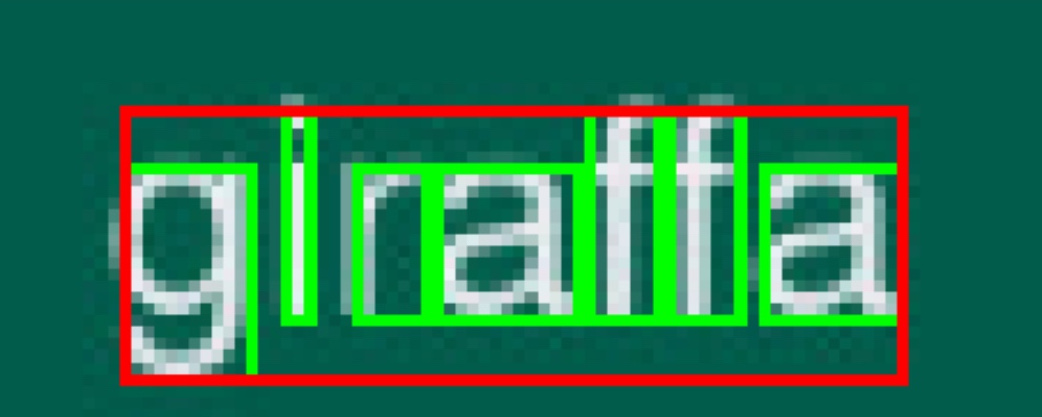
\includegraphics[width=0.3\textwidth]{images/giraffa-bb.jpeg}
	\caption{Individuazione Bounding Box}
	\label{fig:screenshot}
\end{figure}

\section{Fase 2: Classificazione del carattere}

Per la classificazione del carattere viene utilizzato un modello di deep learning. La rete è una Convolutional Neural Network: è composta da 2 layer convoluzionali, ognuno dei quali è seguito da un layer di pooling e da una funzione di attivazione ReLU. Dopo i layer convoluzionali, la rete è composta da tre layer fully connected, che producono l'output finale. Per evitare l'overfitting riscontrato sperimentalmente durante l'addestramento, viene utilizzato il dropout tra i layer fully connected. Il modello è stato addestrato su un dataset di immagini di caratteri e simboli in stampatello, con una risoluzione di 28x28 pixel. È quindi necessario ridimensionare i caratteri estratti dalla fase 1 prima di applicare l'inferenza. Il dataset viene approfondito nella sezione \ref{sec:dataset}.


Fornendo al modello esclusivamente il carattere ridimensionato, di quest'ultimo verrebbero ignorate la dimensione e la posizione all'interno della parola. Questa semplificazione causerebbe problemi nella classificazione della punteggiatura e di caratteri \emph{confondibili}.

Senza informazioni sulla posizione, il modello non sarebbe in grado di distinguere tra `,` e `'`. Inoltre, non sarebbe in grado di distinguere tra maiuscole e minuscole \emph{confondibili}.
\newline

Per carattere \emph{confondibile} si intende una lettera in cui la rappresentazione in stampatello minuscolo coincide con quella in stampatello maiuscolo, se ridimensionata. Ad esempio, `C` e `c` sono caratteri confondibili, così come `S` e `s`, mentre `A` e `a` non lo sono.
L'insieme dei caratteri confondibili maiuscoli ($\text{CI}$) è definito come segue:
$$\text{CI} = \{C, J, K, O, P, S, U, V, W, X, Z\}$$

Ovviamente la controparte minuscola contiene gli stessi caratteri.

\subsection{Utilizzo del Bounding Box globale}

È possibile utilizzare il bounding box globale per fornire al modello informazioni sulla posizione e la dimensione del carattere all'interno della parola. Partendo dal bounding box del carattere e da quello globale, è possibile estrarre il margine superiore e inferiore del carattere rispetto al bounding box globale. Una volta normalizzati rispetto all'altezza del bounding box globale, il margine superiore e inferiore del carattere possono essere utilizzati come due parametri aggiuntivi per il modello.

Con questo accorgimento, il modello è adesso in grado distinguere tra `,` e `'`. Inoltre, nel caso della parola `Bob`, è in grado di classificare correttamente la `o`. Questo è possibile in quanto il margine superiore della `o` è solo presente nel caso in cui il carattere sia maiuscolo.

\subsection{La necessità di euristiche}

Nonostante quest'ultimo approccio possa sembrare efficace, non è sempre in grado di distinguere tra maiuscole e minuscole.
Mostriamo il motivo attraverso un esempio e lo formalizziamo successivamente.
Consideriamo due parole d'esempio:
\begin{itemize}
	\item `Cocco`: la prima lettera non ha margine superiore e inferiore, e deve essere classificata come maiuscola.
	\item `cocco': la prima lettera non ha margine superiore e inferiore, e deve essere classificata come minuscola.
\end{itemize}

Il modello non è quindi in grado di classificare correttamente i caratteri confondibili quando hanno la stessa altezza del bounding box globale.
È necessario utilizzare un'euristica che, confrontando l'altezza dei vari caratteri, sia in grado di `correggere` la forma maiuscola o minuscola del carattere.

Guardando la distribuzione dei caratteri rispetto al loro margine superiore, è possibile notare quando è possibile classificare con certezza i caratteri confondibili.

\begin{figure}[H]
	\centering
	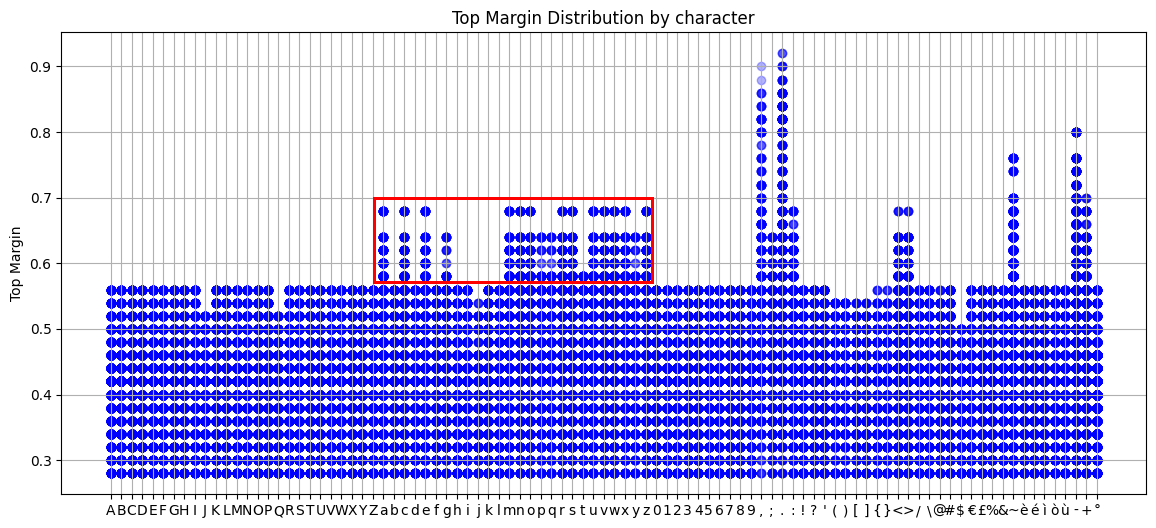
\includegraphics[width=1\textwidth]{images/top_margin_distribution_highlight.png}
	\caption{Distribuzione dei caratteri rispetto al margine superiore. Il rettangolo rosso evidenzia i caratteri confondibili identificabili con affidabilità.}
	\label{fig:top_margin_distribution_highlight.png}
\end{figure}

Rimane comunque il fatto che parole come `COCCO' e `cocco' rimangono indistinguibili anche all'occhio umano, se non affiancate da altre parole che possano disambiguare.

\subsection{L'applicazione dell'euristica}

Data una determinata immagine, per carattere \emph{affidabile} intendiamo un carattere non confondibile oppure un carattere confondibile di forma minuscola con margine superiore significativo. Un carattere è quindi affidabile quando la sua interpretazione agli occhi del modello è priva di ambiguità.

L'euristica per la correzione di maiuscole e minuscole può essere applicata solo quando è presente un carattere confondibile la cui altezza coincide con quella del bounding box globale. In questo caso, l'euristica confronta l'altezza del carattere con quella degli altri caratteri affidabili della parola.
L'unico caso in cui l'altezza di un carattere confondibile coincide con quella del bounding box globale è quando non sono presenti caratteri che aumentano l'altezza del bounding box globale. Tra questi sono inclusi tutti i caratteri maiuscoli e qualche carattere minuscolo, come `b`, `d` e `h`.
Purtroppo però nella pratica le cose non funzionano. Questo avviene in quanto in ogni font i caratteri minuscoli hanno una proporzione di altezza diversa rispetto ai caratteri maiuscoli. Per questo motivo, l'euristica viene applicata sempre, se possibile, ovvero se è presente almeno un carattere affidabile.

\chapter{Dataset}

Essendo il problema dell'OCR uno dei più studiati in ambito di Computer Vision, esistono diversi dataset pubblici che possono essere utilizzati per addestrare e testare i modelli. Tuttavia, la maggior parte di questi dataset sono stati creati per risolvere problemi generali e non sono specifici per il riconoscimento di testi contenuti in screenshot. Per questo motivo, è stato necessario creare una coppia di dataset ad hoc per il problema in questione.

In particolare, essendo l'algoritmo diviso in due fasi, avere due dataset distinti consente di poter valutare in modo individuale ognuna delle due fasi, consentendo di valutare l'accuratezza del modello in modo più preciso.

I due dataset creati sono i seguenti:
\begin{itemize}
	\item \textbf{Dataset dei simboli singoli}: contiene immagini di singoli simboli, che consente di testare esclusivamente la fase di classificazione del singolo carattere.
	\item \textbf{Dataset degli screenshot}:  contiene immagini di screenshot contenenti una sequenza di simboli casuali. Questo consente di testare la pipeline nella sua interezza, comprendendo sia la suddivisione in caratteri che la classificazione del singolo carattere.
\end{itemize}

\section{Dataset dei simboli singoli}

Questo dataset è utilizzato per addestrare il modello di classificazione del singolo carattere. Viene inoltre utilizzato per estrarre delle metriche di valutazione della fase di classificazione, in modo da poter valutare l'accuratezza del modello.

I caratteri considerati nel dataset comprendono quelli dell'alfabeto latino in stampatello maiuscolo e minuscolo, le cifre da 0 a 9 e i seguenti simboli di punteggiatura:

\begin{center}
, ; . : ! ? ' ( ) [ ] \{ \} \textless{} \textgreater{} / \textbackslash{} @ \# \$ \texteuro{} \textsterling{} \% \& \textasciitilde{} à è é ì ò ù - + °
\end{center}

In totale, il dataset contiene 96 classi.

Sono stati presi in considerazione 58 font differenti, ognuno con caratteristiche diverse (ad esempio, grassetto, sottile, italic, ecc.).

È stata generata un'immagine per ogni simbolo, per ogni font. La dimensione considerata è di 28x28 pixel, in modo da essere compatibile con il modello di classificazione utilizzato nella fase 2.

Per la generazione di ogni immagine è stato utilizzato Pillow, una libreria Python per la manipolazione delle immagini. Ogni immagine è stata generata con uno sfondo nero e il simbolo in bianco (con scala di grigi per i bordi). Per come vengono estratti i caratteri dall'immagine da classificare, è necessario che il simbolo nel dataset non abbia margini e che il suo bounding box coincida con il quadro dell'immagine. Per garantire questo vincolo, l'immagine viene inizialmente generata in un'immagine di dimensioni più grandi, successivamente il simbolo viene centrato all'interno dell'immagine e stampato con una dimensione del font arbitraria (grande abbastanza da far entrare il simbolo nel quadro). Dall'immagine viene dunque estratto un bounding box che viene poi ridimenzionato, in modo da ottenere un'immagine di dimensioni 28x28 pixel.
\begin{figure}[H]
	\centering
	
\includegraphics[width=0.3\textwidth]{images/dataset-symbols.png}
	\caption{Esempio di simboli singoli del dataset.}
	\label{fig:dataset-symbols}
\end{figure}

\subsection{Permutazioni di margini}

Come menzionato precedentemente, il modello di classificazione utilizza, oltre al bounding box del simbolo, anche i margini superiore e inferiore del simbolo rispetto al bounding box globale dell'intera parola. Per questo motivo è necessario che il dataset contenga questa informazione per far sì che il modello possa apprendere le relazioni tra il simbolo e il bounding box globale.
\\ \\
L'approccio utilizzato è il seguente, per ogni font:
\begin{itemize}
	\item Si scelgono dimensione di font e quadro dell'immagine arbitrari, font sufficientemente piccolo e quadro abbastanza grande da consentire a qualsiasi simbolo stampato di entrare all'interno dell'immagine.
	\item Si genera un'immagine quadrata per ogni simbolo, con il simbolo centrato all'interno dell'immagine.
	\item Si calcolano, per ogni simbolo, i margini superiore e inferiore del simbolo rispetto al quadro dell'immagine.
	\item Si normalizzano i margini rispetto all'altezza del quadro dell'immagine, in modo da ottenere valori compresi tra 0 e 1.
	\item Vengono create delle permutazioni dei margini, in modo che nel dataset sia presente ogni possibile combinazione di margini per ogni simbolo.
\end{itemize}

Il dataset finale conterrà quindi un simbolo per ogni font, con le varie combinazioni di margini.  Nel caso dei font considerati, il dataset contiene un totale di 179292 tuple.

È importante notare che a causa di questa ultima aggiunta il dataset dei simboli singoli non rimane perfettamente bilanciato: non tutte le classi (simboli) sono rappresentate dallo stesso numero di campioni. Ad esempio, le parentesi tonde (\texttt{(} e \texttt{)}) sono presenti con circa 600 campioni ciascuna, mentre il trattino (\texttt{-}) conta circa 5000 campioni.

Il dataset è stato suddiviso in due sottoinsiemi: train e test. La suddivisione è stata effettuata secondo una proporzione 75\% per il training e 25\% per il test, necessario per la valutazione delle prestazioni del modello.

\subsection{Struttura del dataset}

Il dataset si compone di una serie di cartelle, una per ogni font, contenenti le immagini dei simboli. Ogni cartella è denominata con il nome del font e contiene le immagini dei simboli in formato PNG. I nomi delle immagini contengono il nome del simbolo rappresentato. Sullo stesso livello della cartella del font, sono presenti due file CSV: uno per il training e uno per il test. Questi file contengono l'elenco dei campioni, con la seguente struttura:
\begin{center}
(font, immagine, simbolo, margine\_superiore (\%), margine\_inferiore (\%))
\end{center}

\section{Dataset degli screenshot}
\label{sec:dataset_screenshots}

Il dataset degli screenshot è stato creato per testare l'intera pipeline, dalla suddivisione in caratteri alla classificazione del singolo carattere. Il suo unico scopo è quello di testare l'accuratezza della pipeline per poterne valutare le prestazioni. 

Il dataset contiene immagini di screenshot contenenti una sequenza di 10 simboli casuali. In aggiunta ai simboli considerati nel dataset dei simboli singoli, sono stati aggiunti i caratteri "spazio" e "virgolette" (`"`), in modo da poter testare le euristiche relative al riconoscimento di questi caratteri.

Per la generazione di ogni immagine viene utilizzato un approccio simile a quello utilizzato per il dataset dei simboli singoli. Viene utilizzato Pillow per generare gli screenshot sintetici, scegliando un font casuale e stampando al suo interno la sequenza di simboli da testare.
Per aumentare la precisione delle metriche, vengono inoltre selezionati dei colori casuali per il testo e lo sfondo, in modo da simulare screenshot reali e verificare che le operazioni di pre-processing siano efficaci.

Sono state previste due varianti del dataset, in modo da poter testare la pipeline in modo più completo e verificare che le euristiche implementate funzionino correttamente.

\begin{itemize}
	\item \textbf{Sequenze di 10 simboli casuali}: prevede immagini di sequenze di 10 caratteri estratti randomicamente e concatenati per formare una parola (o una frase, considerando che lo spazio è incluso tra i simboli stampati).
	\item \textbf{Frasi di senso compiuto}: contiene immagini di screenshot di frasi di senso compiuto, estratte da un dataset pubblico di citazioni in lingua inglese. In particolare, le frasi sono state selezionate da un dataset pubblico disponibile su Hugging Face \footnote{Abir ELTAIEF, \textit{english\_quotes (Revision \texttt{7b544c4})}, 2023. Disponibile su: \url{https://huggingface.co/datasets/Abirate/english_quotes}, DOI: 10.57967/hf/1053.}
\end{itemize}




\chapter{Modello di Classificazione}

Per la classificazione dei caratteri estratti dalla fase 1, è stato sviluppato un modello di deep learning. La rete è una Convolutional Neural Network: è composta da 2 layer convoluzionali, ognuno dei quali è seguito da un layer di pooling e da una funzione di attivazione ReLU. Dopo i layer convoluzionali, la rete è composta da tre layer fully connected, che producono l'output finale. Per evitare l'overfitting riscontrato sperimentalmente durante l'addestramento, viene utilizzato il dropout tra i layer fully connected.

\textcolor{red}{img schema + numero epoche}



\chapter{Metodi}
\chapter{Valutazione}
L'obiettivo principale è stato duplice: da un lato valutare la capacità di riconoscimento a livello di singolo carattere, dall'altro quantificare la qualità complessiva della trascrizione a livello di parola. Per ciascun livello di analisi sono state scelte metriche particolari in grado di fornire una misura oggettiva delle performance del modello.

\section{Valutazione a livello di carattere}
\label{sec:valutazione-caratteri}
La valutazione sui singoli caratteri si articola in due diverse analisi:
\begin{itemize}
    \item Curve Precision-Recall
    \item Matrice di confusione
\end{itemize}

\subsection{Curve Precision–Recall}
Le curve Precision-Recall (PR) consentono di analizzare il bilanciamento tra \emph{precision} e \emph{recall} nelle predizioni del modello, mostrando quanto esso riesca a mantenere alta la precisione man mano che aumenta la quantità di caratteri correttamente riconosciuti. Un indicatore sintetico della qualità complessiva è l'area sotto la curva (AUC-PR), che risulta tanto più elevata quanto migliore è la capacità del modello di conciliare accuratezza e sensibilità nel riconoscimento dei caratteri.

\subsubsection{Risultati}
In Figura~\ref{fig:pr_curves} sono riportate le curve per un sottoinsieme rappresentativo di classi non confondibili.

\textcolor{red}{RIFARE screen dopo fixes}

\begin{figure}[htbp]
    \centering
    \begin{subfigure}[t]{0.32\textwidth}
        \centering
        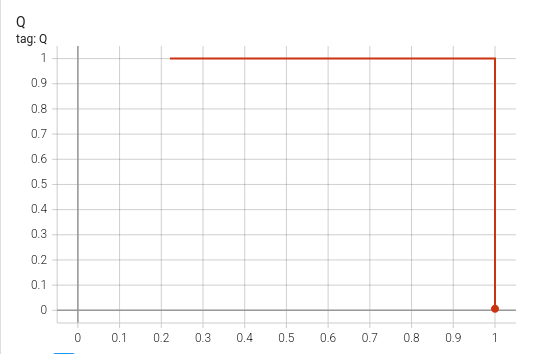
\includegraphics[width=\textwidth]{images/pr_curve1.png}
        \caption{PR-curve \{'\}}
    \end{subfigure}
    \begin{subfigure}[t]{0.32\textwidth}
        \centering
        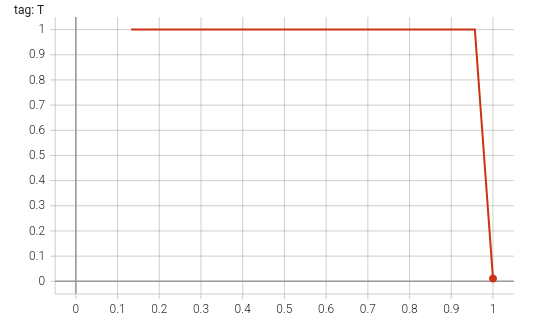
\includegraphics[width=\textwidth]{images/pr_curve2.png}
        \caption{PR-curve \{T\}}
    \end{subfigure}
    \begin{subfigure}[t]{0.32\textwidth}
        \centering
        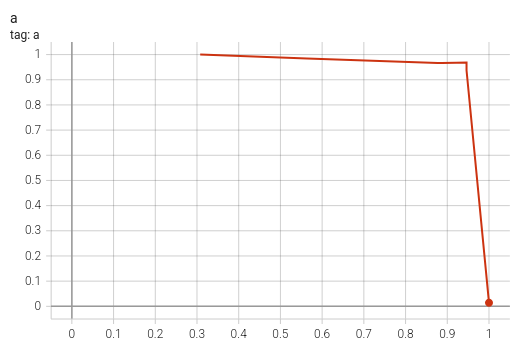
\includegraphics[width=\textwidth]{images/pr_curve3.png}
        \caption{PR-curve \{Y\}}
    \end{subfigure}
    \caption{PR-curves per caratteri non confondibili}
    \label{fig:pr_curves}
\end{figure}

Nel complesso, il modello mostra buone prestazioni, con curve PR ampie e stabili per la maggior parte delle classi.

Tuttavia, alcune classi risultano più problematiche. Come visibile in Figura~\ref{fig:pr-confondibili}.

\begin{figure}[htbp]
    \centering
    \begin{subfigure}[t]{0.32\textwidth}
        \centering
        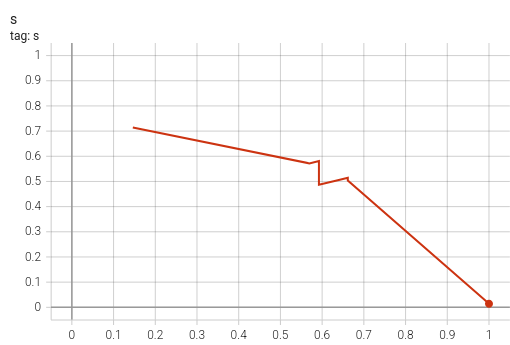
\includegraphics[width=\textwidth]{images/pr_curve_conf1.png}
        \caption{PR-curve \{s\}}
    \end{subfigure}
    \begin{subfigure}[t]{0.32\textwidth}
        \centering
        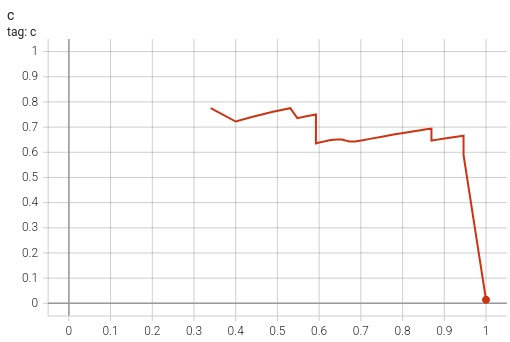
\includegraphics[width=\textwidth]{images/pr_curve_conf2.png}
        \caption{PR-curve \{c\}}
    \end{subfigure}
    \begin{subfigure}[t]{0.32\textwidth}
        \centering
        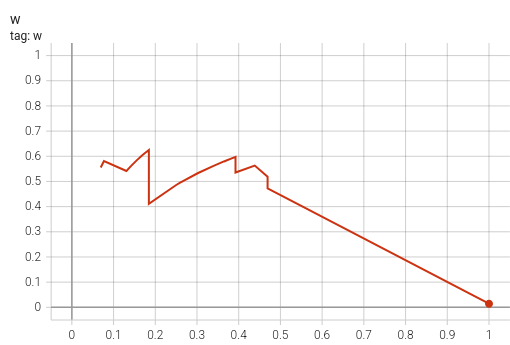
\includegraphics[width=\textwidth]{images/pr_curve_conf3.png}
        \caption{PR-curve \{v\}}
    \end{subfigure}
    \caption{PR-curves per caratteri confondibili}
    \label{fig:pr-confondibili}
\end{figure}

Per valutare l'impatto della distinzione tra maiuscole e minuscole, è stata ripetuta l'analisi ignorando il case. Come mostrato in Figura~\ref{fig:pr-ignore}, l'area sotto la curva migliora sensibilmente, suggerendo che una parte consistente degli errori è dovuta a una difficoltà del modello nel distinguere il case piuttosto che a un'incapacità di riconoscere la forma del carattere.

\begin{figure}[htbp]
    \centering
    \begin{subfigure}[t]{0.32\textwidth}
        \centering
        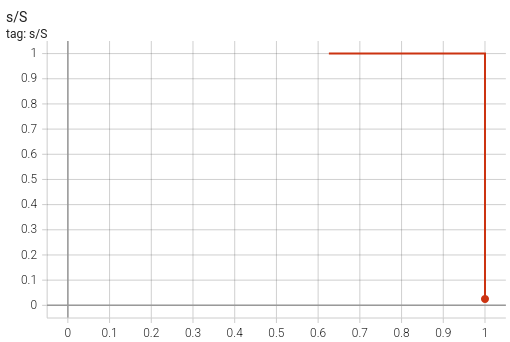
\includegraphics[width=\textwidth]{images/pr_ignore1.png}
        \caption{PR-curve \{s/S\}}
    \end{subfigure}
    \begin{subfigure}[t]{0.32\textwidth}
        \centering
        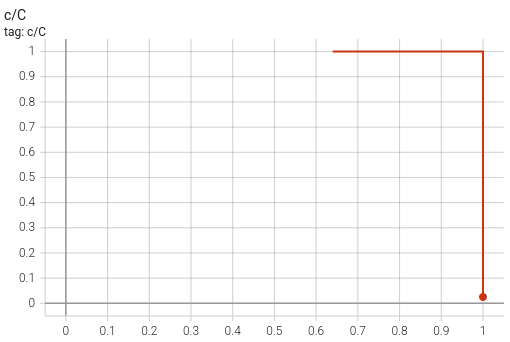
\includegraphics[width=\textwidth]{images/pr_ignore2.png}
        \caption{PR-curve \{c/C\}}
    \end{subfigure}
    \begin{subfigure}[t]{0.32\textwidth}
        \centering
        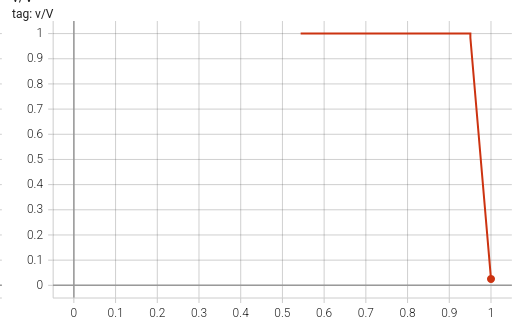
\includegraphics[width=\textwidth]{images/pr_ignore3.png}
        \caption{PR-curve \{v/V\}}
    \end{subfigure}
    \caption{PR-curves ignorando il case}
    \label{fig:pr-ignore}
\end{figure}

Questi risultati suggeriscono che, pur in presenza di buone prestazioni globali, il modello potrebbe beneficiare delle euristiche di post-processing.


\subsection{Matrice di confusione}
La matrice di confusione aggregata a livello di carattere, mostrata in Figura~\ref{fig:confusion_matrix}, offre una panoramica dettagliata sugli errori di classificazione del modello. Ogni cella \((i, j)\) della matrice rappresenta il numero di volte in cui un carattere \(i\) è stato classificato dal modello come appartenente alla classe \(j\).

\begin{figure}[htbp]
    \centering
    \includegraphics[width=0.65\textwidth]{images/confusion_matrix.png}
    \caption{Matrice di confusione}
    \label{fig:confusion_matrix}
\end{figure}

Si osserva come la diagonale principale della matrice sia in gran parte ben marcata, indicando una prevalenza di classificazioni corrette. Le deviazioni più evidenti dalla diagonale si concentrano invece in corrispondenza di coppie di caratteri visivamente simili, che il modello tende a confondere con maggiore frequenza.

Questa osservazione conferma la precedente analisi delle PR-curves: la maggior parte degli errori è riconducibile a un numero limitato di classi particolarmente confondibili.

\section{Valutazione parole}
\label{sec:valutazione-parole}

Per l'analisi a livello di parola sono state adottate due metriche principali:
\begin{enumerate}
    \item Distanza di edit (\emph{Levenshtein distance});
    \item Word Accuracy.
\end{enumerate}

I calcoli sono stati effettuati sui dataset degli screenshot descritti nella \autoref{sec:dataset_screenshots}, che comprendono due tipologie di dati:
\begin{itemize}
    \item sequenze di 10 simboli casuali;
    \item frasi di senso compiuto.
\end{itemize}

\subsection{Distanza di edit}

La distanza di edit\footnote{V. I. Levenshtein, “Binary codes capable of correcting deletions, insertions and reversals,” \textit{Soviet Physics Doklady}, vol. 10, pp. 707–710, 1966.} tra la parola riconosciuta e la parola ground-truth è stata calcolata per ciascun esempio, normalizzando il valore sulla lunghezza della parola.

Di seguito si riporta una tabella con le statistiche principali (media, mediana e deviazione standard) della distanza di edit normalizzata, calcolate separatamente per i due dataset.

\textcolor{red}{INSERIRE valori reali dopo fix errori}

\begin{table}[htbp]
    \centering
    \begin{tabular}{lccc}
        \toprule
        Dataset & Mean & Median & Std \\
        \midrule
        Sequenze casuali & 0.00 & 0.00 & 0.00 \\
        Frasi di senso compiuto & 0.00 & 0.00 & 0.00 \\
        \bottomrule
    \end{tabular}
    \caption{Statistiche della distanza di edit normalizzata per i due dataset}
    \label{tab:edit_distance_stats}
\end{table}

Dal confronto emerge che il modello si comporta meglio nel riconoscimento delle sequenze casuali rispetto alle frasi di senso compiuto. Ciò può essere dovuto a diversi fattori, tra cui:

\textcolor{red}{DIRE quale può essere il motivo}

\subsection{Word Accuracy}
La word accuracy è definita come la percentuale di parole riconosciute esattamente:
\[
    \mathrm{WordAccuracy} = \frac{\text{numero di parole perfettamente riconosciute}}{\text{numero totale di parole}}.
\]

Per una valutazione più dettagliata, sono state considerate tre varianti di word accuracy, che tengono conto di diverse esigenze di confronto:

\begin{itemize}
    \item \textbf{Accuracy case sensitive (CS)}: confronto rigoroso che distingue tra maiuscole e minuscole;
    \item \textbf{Accuracy case insensitive (CI)}: confronto che ignora le differenze tra maiuscole e minuscole, utile per valutare la capacità di distinguere caratteri simili o confondibili;
    \item \textbf{Accuracy case insensitive senza spazi (CSNS)}: confronto che ignora sia il case sia gli spazi, utile per gestire eventuali errori di segmentazione o spaziatura
\end{itemize}

La tabella seguente riporta i valori di word accuracy per ciascuna casistica, calcolati separatamente sui due dataset degli screenshot.

\textcolor{red}{INSERIRE valori reali dopo fix errori}

\begin{table}[htbp]
    \centering
    \begin{tabular}{lccc}
        \toprule
        Dataset & CS & CI & CSNS \\
        \midrule
        Sequenze casuali & 0.00 & 0.00 & 0.00 \\
        Frasi di senso compiuto & 0.00 & 0.00 & 0.00 \\
        \bottomrule
    \end{tabular}
    \caption{Word Accuracy per dataset e casistica di confronto}
    \label{tab:word_accuracy_stats}
\end{table}

\chapter{Demo}
Per illustrare il funzionamento dell'algoritmo insieme ai suoi principali passaggi, è stata realizzata una demo utilizzando la libreria Python \texttt{Gradio}, che consente la creazione di applicazioni web semplici ed intuitive per modelli di machine learning e intelligenza artificiale, in poche righe di codice.

L'interfaccia guida l'utente attraverso tre fasi fondamentali: caricamento dell'immagine, pre-processing e riconoscimento (OCR).

Nella prima fase, l’utente può caricare uno screenshot da elaborare, tramite upload oppure incollandolo direttamente dagli appunti.
\begin{figure}[H]
    \centering
    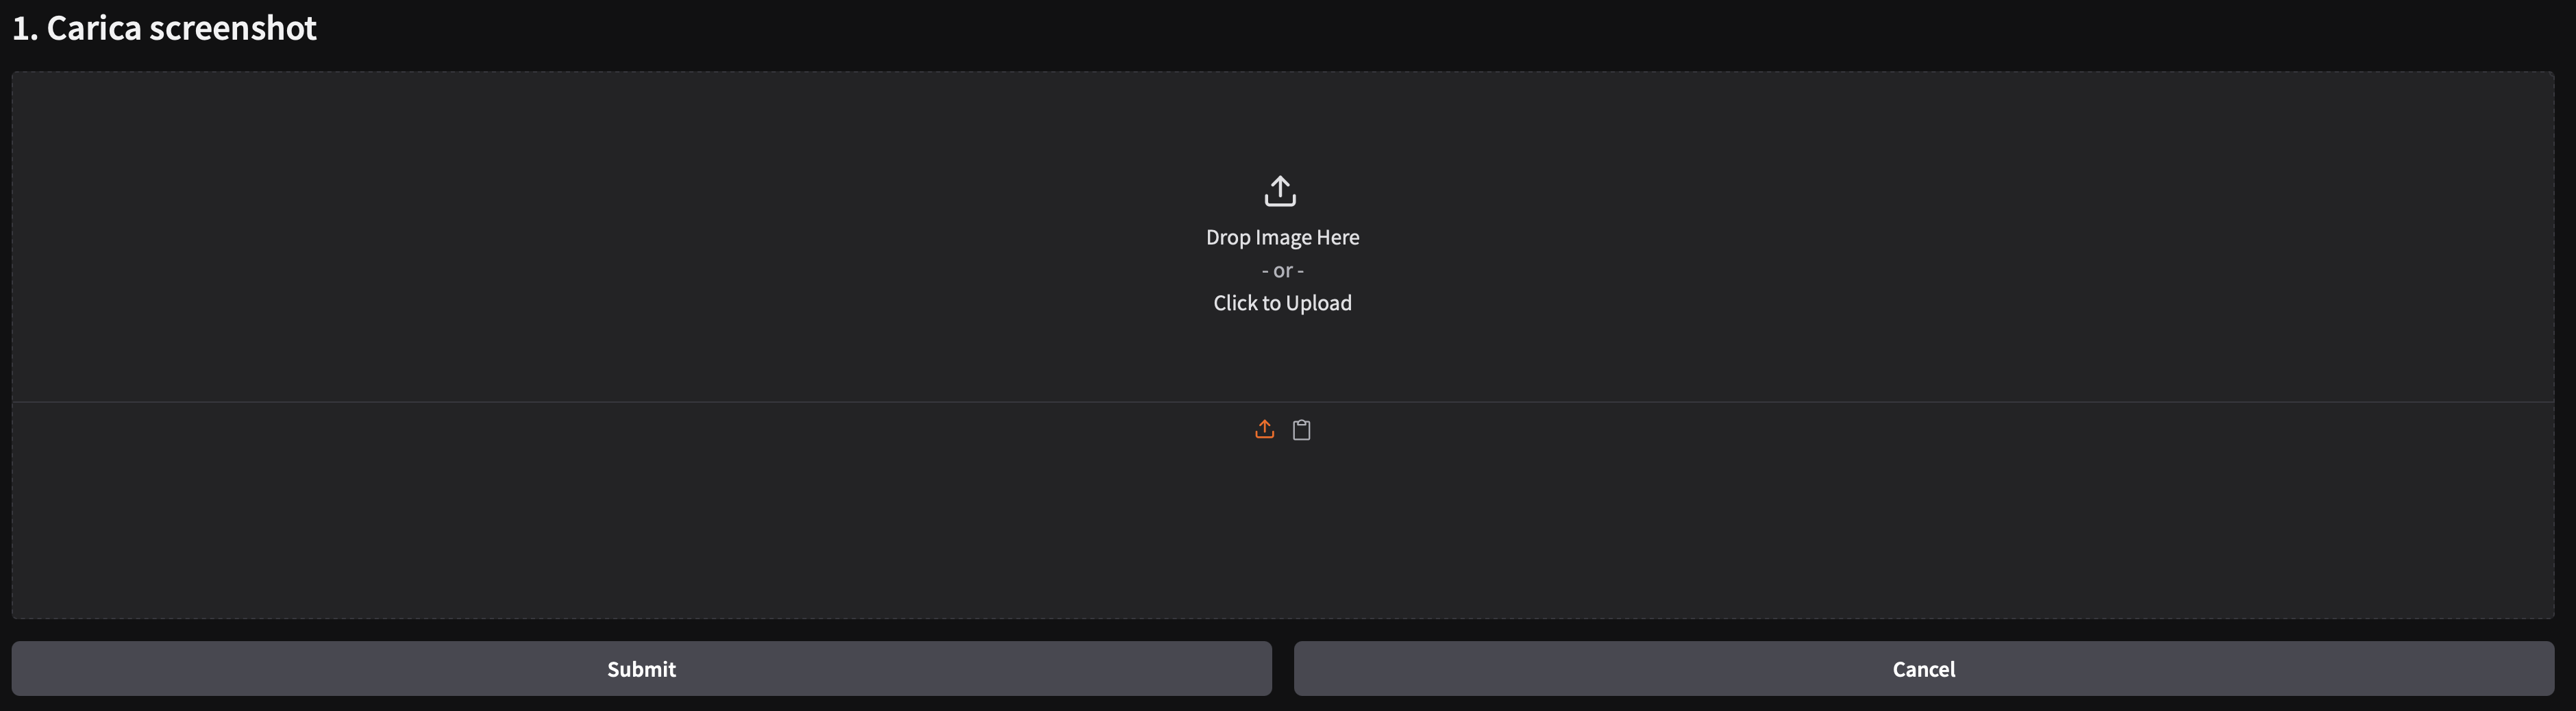
\includegraphics[width=1\textwidth]{images/demo-1fase.png}
    \caption{Interfaccia di caricamento dell'immagine nella demo.}
    \label{fig:demo-1fase}
\end{figure}

Una volta cliccato il pulsante \texttt{Elabora}, avviene l'elaborazione dell'immagine. In output, l'applicazione restituisce due risultati: l'immagine annotata con i bounding box rilevati durante il pre-processing (sovrapposti all'immagine originale) e il testo riconosciuto.

\begin{figure}[H]
    \centering
    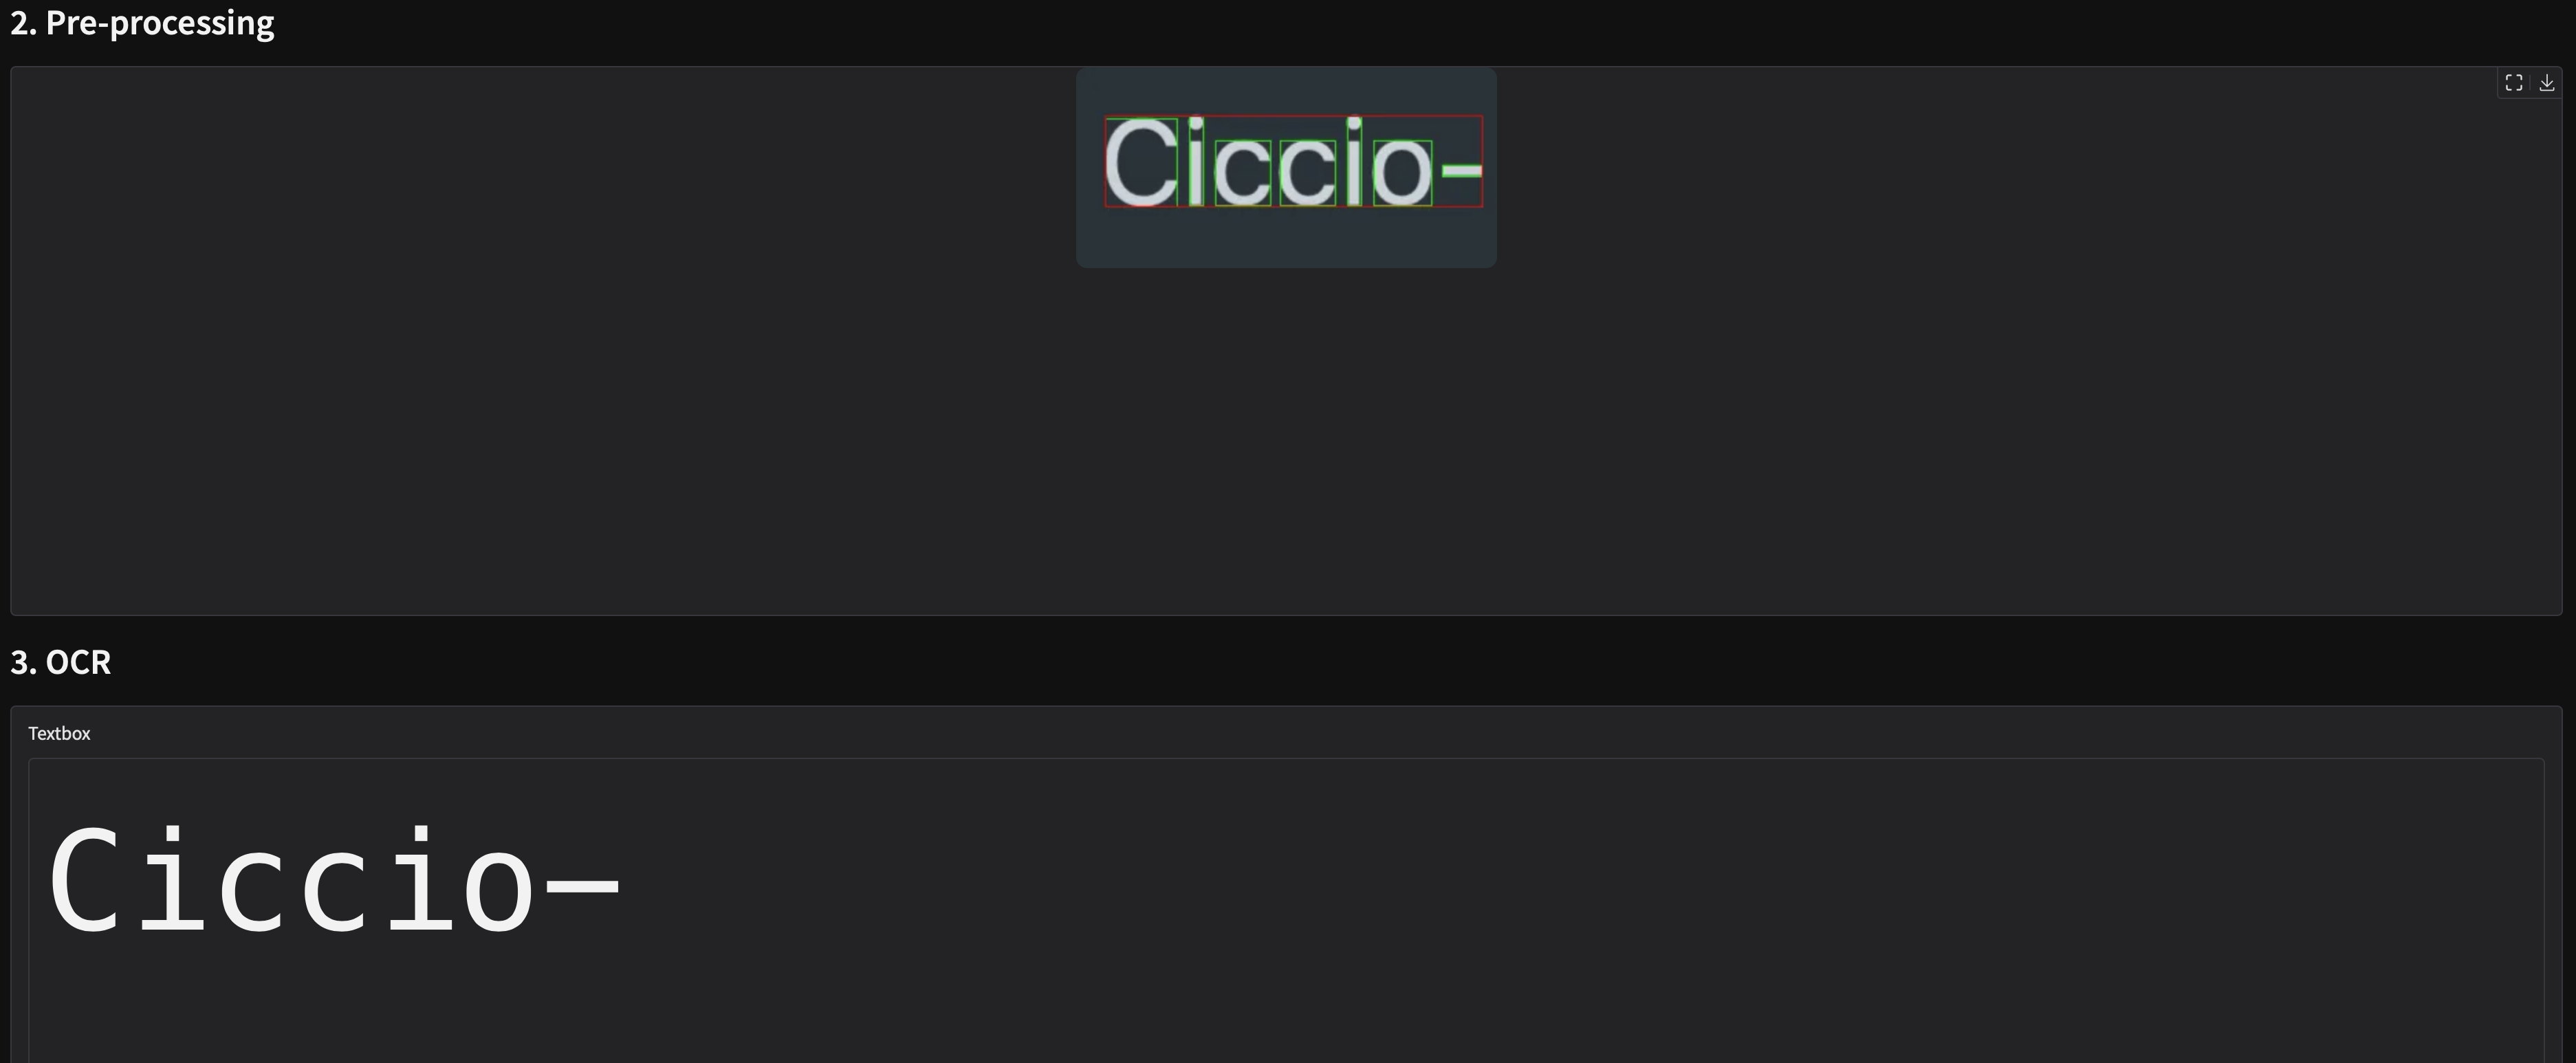
\includegraphics[width=1\textwidth]{images/demo-23fase.png}
    \caption{Output dell'immagine preprocessata e del testo riconosciuto.}
    \label{fig:demo-23fase}
\end{figure}


\chapter{Codice}
\begin{figure}[H]
    \centering
    \tikzstyle{every node}=[draw=black, thick, anchor=west]
    \tikzstyle{selected}=[draw=red, fill=red!30]
    \tikzstyle{optional}=[dashed, fill=gray!50]

\tikzstyle{every node}=[draw=black,thick,anchor=west]
\tikzstyle{selected}=[draw=red,fill=red!30]
\tikzstyle{optional}=[dashed,fill=gray!50]
\begin{tikzpicture}[%
  grow via three points={one child at (0.5,-0.68) and
  two children at (0.5,-0.71) and (0.5,-1.45)},
  edge from parent path={(\tikzparentnode.south) |- (\tikzchildnode.west)}]
  \node {/}
    child { node {core/}
        child{ node {ImageToStringClassifier.py}}
        child{ node {ImageToStringPostprocessing.py}}
        child{ node {ImageToStringPreprocessing.py}}
    }
    child [missing] {}
    child [missing] {}
    child [missing] {}
    child { node {dataset/}
        child { node {dataset.ipynb}}
    }
    child [missing] {}
    child { node {demo/}
        child { node {demo.py}}
    }
    child [missing] {}
    child { node {src/}
        child { node {evaluation\_english\_words.ipynb}}
        child { node {evaluation\_random\_words.ipynb}}
        child { node {ImageToStringNet.py}}
        child { node {main.ipynb}}
    }
    child [missing] {}
    child [missing] {}
    child [missing] {}
    child [missing] {};
\end{tikzpicture}

\section{Core}
La cartella \emph{core} contiene il codice delle tre classi dedicate a preprocessing, classificazione e postprocessing. Ciascun file definisce una classe omonima.

\subsection*{PreProcessing}
La classe \texttt{ImageToStringPreprocessing} prepara l'immagine per la fase successiva di classificazione, segmentando le lettere e normalizzandole in un formato uniforme. A partire da un'immagine in input, esegue operazioni come conversione in scala di grigi, binarizzazione e inversione del contrasto se necessario. 
Successivamente, rileva e raggruppa le componenti connesse per identificare le singole lettere, calcolando anche informazioni spaziali come distanze relative e disegnando le relative bounding box sull'immagine originale.
Ogni lettera viene poi ritagliata, ridimensionata proporzionalmente e centrata su un'immagine nera 28x28, rendendola pronta per le fasi successive. La classe inoltre fornisce metodi per accedere all'immagine segmentata, alle lettere preprocessate e alla loro visualizzazione.


\subsection*{PostProcessing}
La classe \texttt{ImageToStringPostprocessing} a partire dalla lista delle lettere classificate con relative informazioni spaziali, applica le euristiche discusse nei capitoli precedenti per decidere dove inserire spazi tra parole, basandosi sulle distanze orizzontali tra i caratteri. Inoltre, sfrutta la posizione verticale delle lettere rispetto al bounding box generale per correggere l'uso errato delle maiuscole e minuscole nei caratteri confondibili, confrontando ciascun carattere incerto con il primo considerato non confondibile.

\subsection*{Classificazione}
\texttt{ImageToStringClassifier} gestisce l'intero processo di riconoscimento: preprocessing, classificazione caratteri e postprocessing.

\section{Dataset}
La cartella \emph{dataset} contiene il notebook \texttt{dataset.ipynb}, in cui sono descritte e implementate tutte le procedure necessarie per la creazione dei dataset discussi nel Capitolo~\ref{ch:dataset}.

\subsection*{Dataset dei simboli singoli}
Nella prima parte del notebook vengono definite le funzioni per generare automaticamente immagini sintetiche di lettere, variando font e margini \ref{sec:single_dataset}.  
Segue una fase di normalizzazione delle immagini, in cui ciascuna immagine viene convertita in scala di grigi, ridimensionata e centrata su uno sfondo uniforme di 28x28 pixel.

Ad ogni generazione, le informazioni relative all'immagine prodotta — come il percorso, la label di ground truth e le informazioni sui margini — vengono registrate all'interno del file \texttt{dataset.txt}.
A partire da questo file di testo, viene effettuata la suddivisione del dataset negli insiemi di training e test, rispettivamente pari al 75\% e al 25\%.

Il \texttt{DataLoader} farà riferimento a questi file per il caricamento dei dati.

\subsection*{Dataset degli screenshot}
Nella seconda parte è presente la funzione incaricata di generare il dataset degli screenshot \ref{sec:dataset_screenshots}, nelle sue due varianti. La generazione avviene analogamente al dataset dei singoli simboli, variando sempre gli stessi font.
Anche in questo caso, per ogni immagine generata viene prodotto un file di metadati compatibile con il \texttt{DataLoader}.

\section{Demo}
La cartella \emph{demo} contiene il file \texttt{demo.py}, che fornisce l'interfaccia per testare il modello descritta nel Capitolo \ref{cap:demo}. Lo script permette di caricare un'immagine, eseguire il preprocessing, la classificazione e visualizzare il risultato finale.

\section{Src}
La cartella \emph{src} contiene i file principali per l'addestramento, la valutazione e l'esecuzione del modello. In particolare:
\begin{itemize}
    \item \texttt{main.ipynb}
    \item \texttt{ImageToStringNet.py}
    \item \texttt{evaluation\_english\_words.ipynb}
    \item \texttt{evaluation\_random\_words.ipynb}
\end{itemize}

\subsection*{main.ipynb}
Il notebook \texttt{main.ipynb} implementa l'intero workflow di addestramento e valutazione del modello.
All'inizio viene definita la classe \texttt{DigitDataset}, che funge da \texttt{DataLoader} per le fasi di training e testing.

Al fine di effettuare dei test durante il training, il dataset di train viene suddiviso in due sottoinsiemi: training e validation.
Viene quindi inizializzata la rete neurale definita nel file \texttt{ImageToStringNet.py}, insieme alla funzione di loss basata sulla \texttt{CrossEntropy} e all'ottimizzatore \texttt{SGD}.

Per l'addestramento, il flusso è diviso in varie fasi:
\begin{itemize}
    \item \textbf{Gestione configurazioni}
    \item \textbf{Logging Tensorboard}
    \item \textbf{Ciclo di addestramento e validation}
 \end{itemize}

\subsubsection*{Gestione configurazioni}
Le configurazioni da valutare vengono caricate da un file in formato \texttt{.json}, che specifica i parametri di addestramento da testare.  
Ogni configurazione definisce, ad esempio, il tasso di apprendimento, il dropout e il valore di momentum. Per ciascuna configurazione viene istanziata una nuova rete neurale, inizializzata con il tasso di \texttt{dropout} specificato.  
Successivamente, viene configurato un ottimizzatore \texttt{SGD} utilizzando i parametri indicati nella configurazione.  
Nel caso in cui siano già disponibili pesi pre-addestrati per una determinata configurazione, questi vengono caricati automaticamente prima dell'inizio del training.

\subsubsection*{Logging Tensorboard}
Viene creato un writer che registra l'andamento della loss e dell'accuracy durante la fase di addestramento e validation per ogni epoca.

\subsubsection*{Ciclo di training e validation}

Per ogni epoca viene selezionato il \texttt{DataLoader} appropriato in base alla modalità corrente (training o validation).  
Il modello esegue la classificazione dei dati in input e calcola il valore della funzione di loss.  
Nel caso della fase di training, viene eseguita la backpropagation e l'ottimizzazione dei pesi.

Al termine di ciascun batch, i risultati vengono loggati tramite il writer.

Infine, alla fine di ogni epoca, i pesi del modello vengono salvati seguendo uno schema di denominazione standard, che incorpora i principali iperparametri della configurazione corrente.

Le celle successive del notebook sono dedicate alla valutazione del modello, che viene effettuata solo dopo aver trovato i migliori parametri. la valuazione verrà approfondità nel capitolo~\ref{sec:valutazioni}.

\subsection{ImageToStringNet.py}
Il file \texttt{ImageToStringNet.py} contiene la classe che implementa la rete neurale convoluzionale (CNN) utilizzata per la classificazione dei caratteri estratti, discussa nel Capitolo valutazioni~\ref{cap:modello}. 

Il costruttore della classe \texttt{ImageToStringNet} definisce l'architettura della rete, ed è suddiviso in due moduli principali:
\begin{itemize}
    \item \textbf{Feature Extractor}: implementa i due blocchi convoluzionali, dove ciascuno consiste di convoluzione, max pooling e ReLU.
    \item \textbf{Classifier}: prende in input le feature provenienti dal \texttt{feature\_extractor} e le elabora attraverso la rete di tre layer fully connected dove i primi due utilizzano dropout per prevenire l'overfitting seguite da ReLU e l'ultimo layer di output mappa gli 84 neuroni finali al numero di classi possibili.
\end{itemize}

Nel metodo \texttt{forward}, viene definito il flusso dell'input attraverso la rete, l'immagine viene processata dal modulo \texttt{feature$\_$extractor} restituendo un tensore che viene appiattito e vengono concatenati i due margini superiori e inferiori, infine viene passato al modulo \texttt{classifier} che produce l'output finale.

\subsection{Notebook per Evaluation}
I notebook \texttt{evaluation\_english\_words.ipynb} ed \\  \texttt{evaluation\_random\_words.ipynb} sono dedicati alla valutazione delle prestazioni del modello sulle due varianti del dataset degli screenshot. 

In ogni notebook, per ciascuna immagine del dataset associato si esegue il riconoscimento del testo. I risultati ottenuti per ogni immagine vengono raccolti e usati per calcolare una serie di metriche approfondite nel capitolo di valutazione~\ref{sec:valutazioni}.
\chapter{Conclusione}
\end{document}
